\section{Markov Prozesse}
Markov Ketten wurden 1906 von Andrei Andreyvich Markov eingeführt. %missing source
Ein Markov Prozess modelliert ein zeitdiskretes Signal mit einer endlichen Menge an Zuständen.
Dieser Prozess wird beschrieben durch einen Startwahrscheinlichkeitsvektor $\pi$ und eine Transitionsmatrix $A$.
$\pi$ ist die Wahrscheinlichkeit sich in Zeitpunkt $t=0$ in Zustand $i$ zu befinden
und $A_{i,j}$ ist die Wahrscheinlichkeit dass der Prozess sich in Zeitpunkt $t$ in Zustand $j$ befindet 
unter der Bedingung, dass sich der Zustand in Zeitpunkt $t-1$ in Zustand $i$ befand.
Man beobachte, dass die Transitionswahrscheinlichkeiten unabhängig von $t$ sind, so dass der nächste Zustand 
einzig und allein vom gegenwärtigen Zustand des Prozesses anhängt.
Diese Eigenschaft ist bekannt als Markov-Eigenschaft oder Markov-Bedingung.
% Da es sich bei den Werten von \pi und A um Wahrscheinlichkeiten handelt gilt
% x el [0, 1].
Das Ereignis in irgendeinem Zustand zu starten, so wie das Ereignis von einem gegebenen Zustand in irgendeinen anderen Zustand zu wechseln sind sichere Ereignisse.
Somit gelten die Bedingungen, dass die Summe der Startwahscheinlichkeiten $\pi$
und die Summe der ausgehenden Transitionen für jeden Zustand 1 ergeben müssen.

$\sum_{i = 0}^{N} \pi_i = 1 $
$\sum_{j = 0}^{N} A_{i,j} = 1 $

Um das ganze an einem Beispiel zu verdeutlichen stellen wir uns einen Markovprozess vor, welcher 
die durchschnittliche jährliche Temperatur modeliert. Um das Beispiel übersichtlich zu halten beschränken wir uns auf die Zustände Heiß und Kalt.

Die Startwahscheinlichkeiten $\pi$ entsprechen den Wahrscheinlichkeiten, dass ein zufälliger Tag heiß beziehungsweise kalt ist.
Die Transitionswahrscheinlichkeiten seien gegeben durch $A$.
Solch ein Markov Prozess kann anschaulich als gerichteter Transitionsgraph representiert werden.

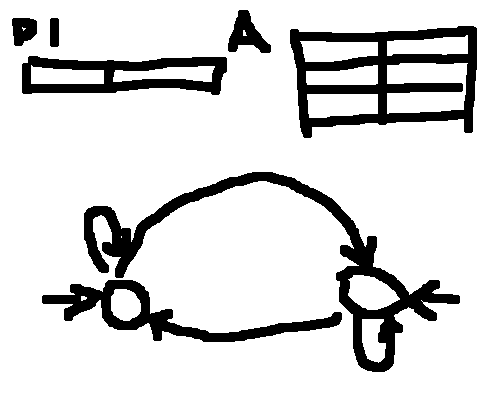
\includegraphics[scale=1.0]{images/Markov_Chain_Example.png}

Mit diesem Modell können wir nun zum Beispiel berechnen, was die Wahrscheinlichkeit ist die Temperaturfolge 
{Heiß, Kalt, Heiß, Kalt, Kalt} zu beobachten unter der Vorraussetzung, dass die gegenwärtige Temperatur Heiß ist.
$O = \{S_1, S_2, S_1, S_2, S_2 \}$
$P(O \mid Model, q_1 = S_1) = P(q_1=S_1 \mid Model) 
\wedge P(S_1 \mid S_1) 
\wedge P(S_2 \mid S_1)
\wedge P(S_1 \mid S_2)
\wedge P(S_2 \mid S_1)
\wedge P(S_2 \mid S_2) $
$= \pi_{1} 
\cdot A_{1,1} 
\cdot A_{1,2} 
\cdot A_{2,1}
\cdot A_{1,2}
\cdot A_{2,2}$
$= 0.8 \cdot 0.4 \cdot 0.3 \cdot 0.7 \cdot 0.5 \cdot 0.3 \cdot 0.9 = 0.009072$

Allgemeiner können wir eine beliebige Observations-Sequenz O berechnen mit 
$O = \{O_1, O_2, \dots, O_{T-1}, O_T \}$
$P(O \mid Model) = \pi_{O_1} \cdot \prod_{t = 2}^{T} A_{O_{t-1}, O_t}$

Ein Prozess kann also nur mit einer Markovkette modeliert werden, wenn wir diesen Prozess beobachten können.
Es kann jedoch sein, dass wir den Prozess selbst nicht beobachten können dann benötigen wir ein 
Hidden Markov Model um diesen zu modellieren.


\section{Hidden Markov Modelle}
Angenommen wir möchten die durchschnittlichen jährlichen Temperaturen 
modellieren für einen Zeitraum bevor es Temperaturaufzeichnungen gab.
Wir können die Temperatur in diesem Fall nicht direkt beobachten.
Es ist jedoch bekannt, dass sich die Temperatur auf das Wachstum von Bäumen auswirkt.
Warme Jahre führen in der Regel zu breiteren Jahresringen und kalte Jahre zu schmaleren.
Die Jahresringe von Bäumen für den gewünschten Zeitraum können wir beobachten.

Seien S, M und L die verschiedenen Breiten an Jahresringen welche beobachtet werden können.
S steht für dünne, M für mittlere und L für breite Jahresringe.
Unser Modell wird nun um eine Emissionsmatrix B erweitert.

Die Wahrscheinlichkeit für eine gegebene Temperatur irgend eine dicke zu Beobachten ist 
ebenfalls ein sicheres ereignis und somit gilt auch für die Reihen von B analog zu A.

$B_{i, k}$ ist die Wahrscheinlichkeit in Zustand i Emissions-Symbol k zu beobachten.
$B_{1, 2}$ gibt die Wahrscheinlichkeit an in in einem Heißen Jahr 
Jahresringe mittlerer Breite zu beobachten.

Mit diesem erweiterten Modell kann man nun folgende Fragen stellen
Problem 1:
Was ist die Wahrscheinlichkeit einer gegebenen Observationssequenz unter einem gegebenen Modell?

Problem 2:
Gegeben eine Observationssequenz und ein Model. Aus welcher Sequenz an Zuständen ist die Observationssequenz 
am Wahrscheinlichsten entstanden?

Problem 3:
Gegeben ein Modell und eine Observationssequenz.
Wie kann man die Wahrscheinlichkeit $P(O \mid \lambda)$ maximieren?



\subsection*{Problem 1}
Wie berechnet man die Wahrscheinlichkeit einer Observationssequenz 
unter einem Modell?
Wenn wir die Abfolge der Zustände haben lässt sich $P(O \mid \lambda)$
sehr einfach berechnen da die Wahrscheinlichkeit ein Symbol k zu beobachten 
unter der Bedingung in Zustand i zu sein nichts anderes ist als $B_{i,k}$
$P(O \mid Q, \lambda) =  \prod_{t=1}^{T} b_{q_t}(O_t)$

Die Wahrscheinlichkeit von $P(O \mid \lambda)$ ist equivalent zu der 
Summe der bedingten Wahrscheinlichkeiten aller möglichen Zustandsfolgen.
$P(O \mid \lambda) = \sum_{all Q} P(O \mid Q, \lambda )$
Es ist möglich $P(O \mid \lambda)$ so zu berechnen, jedoch wächst die 
Anzahl der Möglichen Zustandsabfolgen Q exponentiell in Abhängigkeit von T.
Präzise gesagt gilt $|Q| = 2T \cdot N^T$. Selbst wenn N und T kleine Werte einnehmen
ist die benötigte Rechenleistung untragbar. Für N=5 und T=100
müssten $2 \cdot 100 \cdot 5^{100} \approx 10^{72}$ Berechnungen durchgeführt werden.
Um diese Zahl in Perspektive zu packen $10^{72}$ ist mindestens 3 mal mehr als 1000 und 1000 ist schon ziemlich groß.

\subsection*{Forward Backward Procedure}
Sei alpha die Forwärtsvariable folgendermaßen definiert

$\alpha_t(i) = P(O_1 O_2 \dots O_t \wedge q_t = S_i \mid \lambda)$

$\alpha_t(i)$ Beschreibt also die Wahrscheinlichkeit die partielle Observationssequenz
$O_1 O_2 \dots O_t$ zu beobachten und in Zeitpunkt t in in Zustand i zu sein.

$\alpha_t(i)$ kann folgendermaßen induktiv berechnet werden

Für $t=0$ lässt sich $alpha_t(i)$ aus $\pi$ und $B$ berechnen, da noch keine Transition 
stattgefunden hat. 
$\alpha_0(i) = \pi_i \cdot b_i(O_0)$

Für $t>0$ gilt
$\alpha_{t+1}(j) = \left[ \sum_{i=1}^{N} \alpha_t(i) \cdot a_{i,j} \right] \cdot b_j(O_{t+1})$

Eine effiziente berechnung von $\alpha$ ist möglich aufgrund der Markov-Eigenschaft,
welche besagt, dass der Zustand in Zeitpunkt $t+1$ nur vom Zustand in Zeitpunkt $t$ abhängt.
Für jeden Zeitpunkt und jeden Zustand gibt es genau N Zustände in denen sich
der Prozess zuvor befunden haben kann.
Somit ergibt sich eine Rechenkomplexität von $N^2 \cdot T$


Wahrscheinlichkeit die Partielle Observationssequenz zu beobachten 
hängt von der Wahrscheinlichkeitsverteilung ab in welchem Zustand
sich der Prozess befand nach dem die Partielle Observationssequenz t-1
beobachtet wurde. Da für jeden Zeitpunkt t sich der Prozess in t-1 

Nach der Markov-Eigenschaft gilt, dass der Zustand in Zeitpunkt $t+1$
einzig und allein vom Zustand in Zeitpunkt $t$ abhängt.
Daher ist eine effiziente Berechnung von $\alpha$ möglich, da für

Der Prozess kann sich nach Beobachtung von o...t nur in N Zuständen befinden.
Da wir für jeden Zeitpunkt und für jeden Zustand 


Wichtig ist anzumerken, dass alpha nicht die Wahrscheinlichkeit ist 
in Zeitpunkt t in Zustand i zu sein sondern nur die 
Wahrscheinlichkeit angibt i dunno dawg

Wir führen die Rückwärtsvariable $beta$ ein, welche wie folgt definiert ist.
$\beta_t(i) = P(O_{t+1}, O_{t+2} \dots O_T \mid q_t = S_i, \lambda)$
Somit ist $\beta_t(i)$ die Wahrscheinlichkeit in Zeitpunkt t in Zustand $S_i$ zu sein
und außgehend von $S_i$ die partielle Observationssequenz $O_{t+1}, O_{t+2} \dots O_T$
zu beobachten.
Für t = T gilt
$\forall_i \  1 \leq i \leq N \mid \beta_T(i) = 1  $

Für t < T gilt:
$\beta_t(i) = \sum_{j=1}^{N} a_{i,j} \cdot b_j(O_{t+1}) \cdot \beta_{t+1}(j)$

Mit den Variablen $\alpha$ und $\beta$ gewappnet können wir nun eine weitere Variable definieren.
$\gamma_t(i) = P(q_t = S_i \mid O, \lambda)$
Diese beschreibt die Wahrscheinlichkeit beim Beobachten von O in Zeitpunkt $t$ in Zustand $i$
zu sein. $\gamma_t(i)$ wird berechnet durch
% Warum wird hier die Wahrscheinlichkeit P(O| lamda)
% nicht einfach nur mit alphaT berechnet??
\begin{equation}
\gamma_t(i)
= \frac{\alpha_t(i) \cdot \beta_t(i)}{P(O \mid \lambda)}
= \frac{\alpha_t(i) \cdot \beta_t(i)}{\sum_{i=1}^{N} \alpha_t(i) \cdot \beta_t(i)}
\end{equation}




% \[yeahboiiiiiii\]
% \begin{align}
% \label{yeah boiiiii}    
% \end{align}



\section{Baum Welch Algorithmus}
In den vorherigen Beispiel waren die Werte für die Parameter $\pi$, $A$ und $B$ gegeben.
Häufig sind diese Werte jedoch unbekannt und es liegen ledigich Observationssequenzen vor.









% \section{Hidden Markov Modelle}

% - werden schon seit den späten 1960er Jahren verwendet (Rabiner)

% - Ich werde erklären was ein Hidden Markov Model ist und wie Parameter Estimation funktioniert
% - Dann werde ich auf Metaheuristische Optimierungsverfahren eingehen 


% - Hidden Markov modelle sind eine Weiterentwicklung der Markov Ketten.
% - Mit einem Hidden Markov Modell können wir einen Prozess modellieren, welchen wir selbst nicht messen können
% anhand von Observationen welche von diesem Versteckten Prozess verursacht werden

% co2 konsentration -> Temperatur
% Temperatur -> BaumWachstum


% - Ein Diskretes Hidden Markov ist ein Probabilistischer Zustandsautomat, welcher von drei Parametern beschrieben wird
% - Ein HMM modeliert ein Zeitdiskretes Signal. 
% - die variable t gibt an in welchem Zeitpunkt man sich gerade befindet.

% - Wir können ein Signal Modellieren  
% - Ein Hidden Markov Model heist "hidden" weil wir die Zustände und die Übergangswahrscheinlichkeiten
% nicht kennen. Wir kennen nur die Observationssequenzen.
% - Wenn wir nun solch ein Signal modellieren wollen machen wir die Annahme,
% dass die Observationen durch eine Zugrundeliegenden Prozess verursacht werden, welchen wir 
% jedoch selbst nicht messen können
% - Wir machen die Annahme, dass es einen Prozess gibt welcher die Beobachtungen verursacht


% - Wir observieren die Co2 konzentrationen und machen die Annahme, dass die Co2 konzentrationen durch
% Temperatur Verursacht werden

% - PI ist der Startwahrscheinlichkeitsvektor PI_i ist die Wahrscheinlichkeit in t=0 sich in Zustand i zu befinden
% - B die Emissionswahrscheinlichkeiten. B_i_k ist die Wahrscheinlichkeit Symbol k zu beobachten wenn man sich in Zustand i befindet
% - A die Transitionsmatrix. A_i_j ist die Wahrscheinlichkeit dass der Zustand in t+1 j ist wenn der Zustand in t i ist



% \section{Die Drei Probleme}




% \section{Underflow & Overfitting}

% - Underflow tritt auf wenn Zahlen so klein werden, dass sie den darstellbaren Bereich eines 
% Computers verlassen.
% - Ein typischer Computer hat eine Dynamische Range von ? bis ?


